\documentclass[11pt,a4paper]{article}
\usepackage{fontspec}
\setmainfont{TeX Gyre Pagella}
\newfontfamily\headfont{Inter}[UprightFont=*-ExtraBold,BoldFont=*-ExtraBold,Extension=.otf,Path=/usr/share/fonts/opentype/inter/]
\usepackage[a4paper,margin=2.3cm]{geometry}
\usepackage{graphicx,booktabs,float,caption,array,xcolor,longtable}
\usepackage{xurl}
\usepackage[hidelinks]{hyperref}
\usepackage{titlesec}
\usepackage[round]{natbib}
\usepackage{setspace}
\setstretch{1.05}
\renewcommand{\topfraction}{0.9}
\renewcommand{\bottomfraction}{0.8}
\renewcommand{\textfraction}{0.1}
\renewcommand{\floatpagefraction}{0.75}
\setlength{\parindent}{0pt}
\setlength{\parskip}{0.55em}
\titleformat{\section}{\headfont\Large}{\thesection}{0.8em}{}
\titleformat{\subsection}{\headfont\large}{\thesubsection}{0.8em}{}
\captionsetup{font=small,labelfont=bf}
\urlstyle{same}
\newcommand{\kmq}{km\textsuperscript{2}}
\hypersetup{pdftitle={When the Ice Came South},pdfauthor={Tristan Hotham}}

\begin{document}
\begin{center}
{\Large\bfseries When the Ice Came South\par}
\vspace{0.4em}
{\large The Northern Hemisphere's ice sheets through the Quaternary,\\what lay beneath them and the land the sea gave up\par}
\vspace{1.2em}
{\large Tristan Hotham\par}
\vspace{0.3em}
{\small Independent researcher\\
ORCID: 0000-0003-4931-9349\\
DOI: https://doi.org/10.5281/zenodo.23878610\par}
\vspace{0.8em}
2026
\end{center}

\begin{quote}
\small
\begin{center}\textbf{Abstract}\end{center}
I measure and map the best-estimate reconstructions of Northern Hemisphere ice-sheet extent published by \citet{batchelor} for 18 time slices from the late Gauss Chron (3.59 to 2.6 million years ago) to the Last Glacial Maximum (LGM, about 26,500 years ago), and ask what lies under them today. Measured in an equal-area projection, the largest outline is MIS 6 (132,000 to 190,000 years ago), at 33.8 million \kmq, 29\% more than the LGM (26.2 million \kmq), which ranks 4th of the 18 slices; the authors' own area table gives the same order for the seven largest slices. Together the outlines cover 37.0 million \kmq. The LGM ice covered 97\% of Canada, all of Ireland, Sweden and Finland, and 61\% of the United Kingdom; 709 of the 7,342 cities and towns in Natural Earth, with a combined population figure of about 141 million, stand inside it, New York 13 km inside the edge. London lies outside every outline, 16 km from the MIS 12 edge. The ice reached 37.2°N in North America in MIS 6 and MIS 12 and 48.3°N in Europe in MIS 6. On the ETOPO1 relief, a sea 120 m lower than today exposes 21.2 million \kmq\ of sea floor, 17.5 million of it outside the LGM ice; the largest new lands are the Sahul and Sunda shelves.

\textbf{Keywords:} ice sheets; Quaternary; Last Glacial Maximum; glaciation; sea level; land bridges; Doggerland; Beringia; palaeogeography; open data; mapping
\end{quote}

\section{Introduction}
The ice sheets of the Last Glacial Maximum are familiar from maps of North America and Europe, but they were neither the only nor the largest ice sheets of the Quaternary. \citet{batchelor} compiled the published empirical and modelled evidence for the extent of Northern Hemisphere glaciation and drew minimum, maximum and best-estimate reconstructions of the ice for 18 time slices, from the late Gauss palaeomagnetic Chron to the LGM. Their outlines are published as shapefiles with an area table. This paper uses the best-estimate outlines to answer simple questions: how big was the ice in each slice, how far south did it reach, which of today's countries and cities lay beneath it, and how much land did the lower sea level of a glacial maximum uncover. An interactive map accompanies the paper at \url{https://maps.tristanhotham.com/ice-ages/}.

\section{Data and methods}
\subsection{Ice outlines}
The shapefiles come from the authors' repository on the Open Science Framework (\url{https://osf.io/7jen3/}). The README supplied with them gives the time slices and their ages: the LGM, 30, 35, 40 and 45 ka, MIS 4 (58 to 72 ka), MIS 5a (72 to 86 ka), 5b (86 to 92 ka), 5c (92 to 108 ka), 5d (108 to 117 ka), MIS 6 (132 to 190 ka), MIS 8 (243 to 279 ka), MIS 10 (337 to 365 ka), MIS 12 (429 to 477 ka), MIS 16 (622 to 677 ka), MIS 20 to 24 (790 to 928 ka), the early Matuyama Chron (1.78 to 2.6 Ma) and the late Gauss Chron (2.6 to 3.59 Ma). For the LGM there is one outline, derived mainly from \citet{ehlers}; for every earlier slice there are minimum, maximum and best-estimate outlines. I use only the best estimates; the minimum and maximum enter through the authors' area table. The README states no licence; the repository is released under CC BY 4.0.

All files but one are in a north polar Lambert azimuthal equal-area projection on the WGS84 ellipsoid (centre 90°N, 0°E); the LGM file is in geographic coordinates and was reprojected after adding vertices every 0.05°. I repaired invalid polygons (in 12 files), dissolved each slice to a single outline, and measured areas in the equal-area projection. The files for 45 ka and the late Gauss Chron also contain today's glaciers worldwide, apparently from a global glacier layer, including Antarctica; I keep only parts north of the equator, removing 12.4 million \kmq\ (as projected) from each. For the web map the outlines are generalised to about 7 km; the released outlines, to 1.5 km. The authors' outlines aim to show the largest extent within each slice, except that for 45 ka, MIS 5a and MIS 5c they show the ice at peak warmth. They are not intended for local-scale use, and the authors describe some, notably MIS 8 and MIS 10, as highly uncertain, indicating the likely amount of ice rather than the position of its margin. For regions without evidence, ice was taken from a slice with a similar global $\delta^{18}$O value, and templates were used for Greenland, Iceland, the North American Cordillera and north-east Asia \citep{batchelor}.

\subsection{Countries, places and distances}
Country areas under ice are the intersections of Natural Earth 1:10m countries (Northern Hemisphere parts) with each outline in the same equal-area projection, divided by the whole country's area in the Equal Earth projection. Cities and towns are the 7,342 points of Natural Earth's populated places, each with Natural Earth's population figure (\texttt{pop\_max}, which describes the built-up area), so sums over places are approximate and are not a census. For a list of large cities chosen in advance, I measured the distance from the city centre to the ice edge in an azimuthal equidistant projection centred on the city, which gives true distances on the ellipsoid to the generalised edge. Whether a point is inside is decided in the equal-area projection.

\subsection{Southernmost reach}
For each slice I take the lowest latitude on any outline polygon of 50,000 \kmq\ or more, the authors' threshold for an ice sheet, between 170°W and 50°W (North America) and between 12°W and 60°E (Europe). Mountain glaciers and smaller ice caps are not in the reconstructions.

\subsection{Exposed sea floor}
Sea-floor depths come from ETOPO10, a 10 arc-minute resampling of ETOPO1 \citep{etopo1}, with cell areas on the authalic sphere. Land today is any cell whose ice-surface elevation is above 0 m or which lies inside Natural Earth's land; the sea is every other cell in a water body joined to the world ocean or larger than 50,000 \kmq, except the Caspian Sea, which keeps its own level. This keeps the Black Sea (0.45 million \kmq\ on this grid) and drops the Caspian and lakes. Depth is the bedrock version, so floating ice shelves are not mistaken for shallow sea. A cell is exposed at a sea level $S$ if it is sea today and its floor is at or above $S$. I use $S=-120$ m, near the LGM lowstand of about 120 to 125 m quoted on Wikipedia \citep{wiki}, and $S=-60$ m for comparison. No isostatic adjustment, erosion or sedimentation is modelled, matching the authors' choice to draw the ice on today's topography. Regional figures use boxes I drew round the main shelf seas (Table~\ref{tab:shelves}). Land bridges are tested by whether two of today's landmasses fall in the same connected region of land plus exposed floor; at the grid's resolution of about 18 km, narrow deep straits may be missed, and I report no tests that hinge on them.

\section{Results}
\subsection{Ice area}
Table~\ref{tab:areas} and Figure~\ref{fig:areas} give the area of every slice. The largest outline is MIS 6, 33.8 million \kmq, followed by MIS 12 (32.4 million) and MIS 16 (32.2 million). The LGM, at 26.2 million \kmq, ranks 4th; MIS 6 is 29\% larger (27\% in the authors' table). At the LGM 34.4\% of the ice lay over what is now sea, from Hudson Bay to the Barents Sea. My measured areas are within 4.2\% of the authors' table for every slice except 40 ka, where the outline holds 20\% more ice than the table; the difference lies mostly in ice masses in north-east Asia that the table's ``others'' column does not appear to count. The three slices drawn at peak warmth are the three smallest, none above 7.2 million \kmq. Together the 18 outlines cover 37.0 million \kmq, 41\% more than the LGM; 4.8 million \kmq, about half of it Greenland, is inside all of them.

\begin{table}[tbp]\centering\footnotesize\setlength{\tabcolsep}{4pt}\caption{Ice area by time slice, million \kmq. Measured: the best-estimate outline in an equal-area projection; authors: \citet{batchelor}'s table (best, minimum, maximum). Over sea: share of the measured ice over today's sea.}\label{tab:areas}\begin{tabular}{llrrrrrr}\toprule Slice & Age & Measured & Rank & Authors & Min & Max & \% over sea\\\midrule
LGM & around 26,500 years ago & 26.21 & 4 & 26.42 &  &  & 34.4\\
30 ka & about 30,000 years ago & 14.30 & 10 & 14.30 & 12.56 & 25.04 & 21.6\\
35 ka & about 35,000 years ago & 12.83 & 12 & 12.88 & 11.01 & 24.75 & 20.2\\
40 ka & about 40,000 years ago & 10.65 & 15 & 8.90 & 7.07 & 26.85 & 13.4\\
45 ka & about 45,000 years ago & 7.17 & 16 & 7.48 & 5.14 & 19.20 & 12.5\\
MIS 4 & 58,000 to 72,000 years ago & 23.77 & 5 & 23.64 & 16.90 & 30.79 & 33.1\\
MIS 5a & 72,000 to 86,000 years ago & 6.93 & 18 & 6.94 & 2.42 & 17.62 & 8.5\\
MIS 5b & 86,000 to 92,000 years ago & 12.89 & 11 & 13.22 & 10.18 & 23.76 & 28.5\\
MIS 5c & 92,000 to 108,000 years ago & 6.93 & 17 & 6.67 & 2.42 & 18.26 & 8.5\\
MIS 5d & 108,000 to 117,000 years ago & 12.48 & 13 & 12.84 & 9.26 & 25.93 & 25.5\\
MIS 6 & 132,000 to 190,000 years ago & 33.82 & 1 & 33.65 & 26.30 & 35.73 & 32.7\\
MIS 8 & 243,000 to 279,000 years ago & 23.47 & 6 & 23.62 & 17.36 & 34.55 & 32.1\\
MIS 10 & 337,000 to 365,000 years ago & 21.55 & 9 & 21.81 & 13.91 & 34.15 & 35.2\\
MIS 12 & 429,000 to 477,000 years ago & 32.45 & 2 & 32.52 & 24.02 & 36.47 & 30.5\\
MIS 16 & 622,000 to 677,000 years ago & 32.17 & 3 & 32.04 & 20.06 & 36.62 & 29.1\\
MIS 20 to 24 & 790,000 to 928,000 years ago & 23.08 & 7 & 23.09 & 10.70 & 35.69 & 29.4\\
Early Matuyama & 1.78 to 2.6 million years ago & 21.57 & 8 & 21.77 & 10.52 & 29.10 & 29.9\\
Late Gauss & 2.6 to 3.59 million years ago & 11.07 & 14 & 10.95 & 3.75 & 20.09 & 19.5\\
\bottomrule\end{tabular}\end{table}

\begin{figure}[tbp]\centering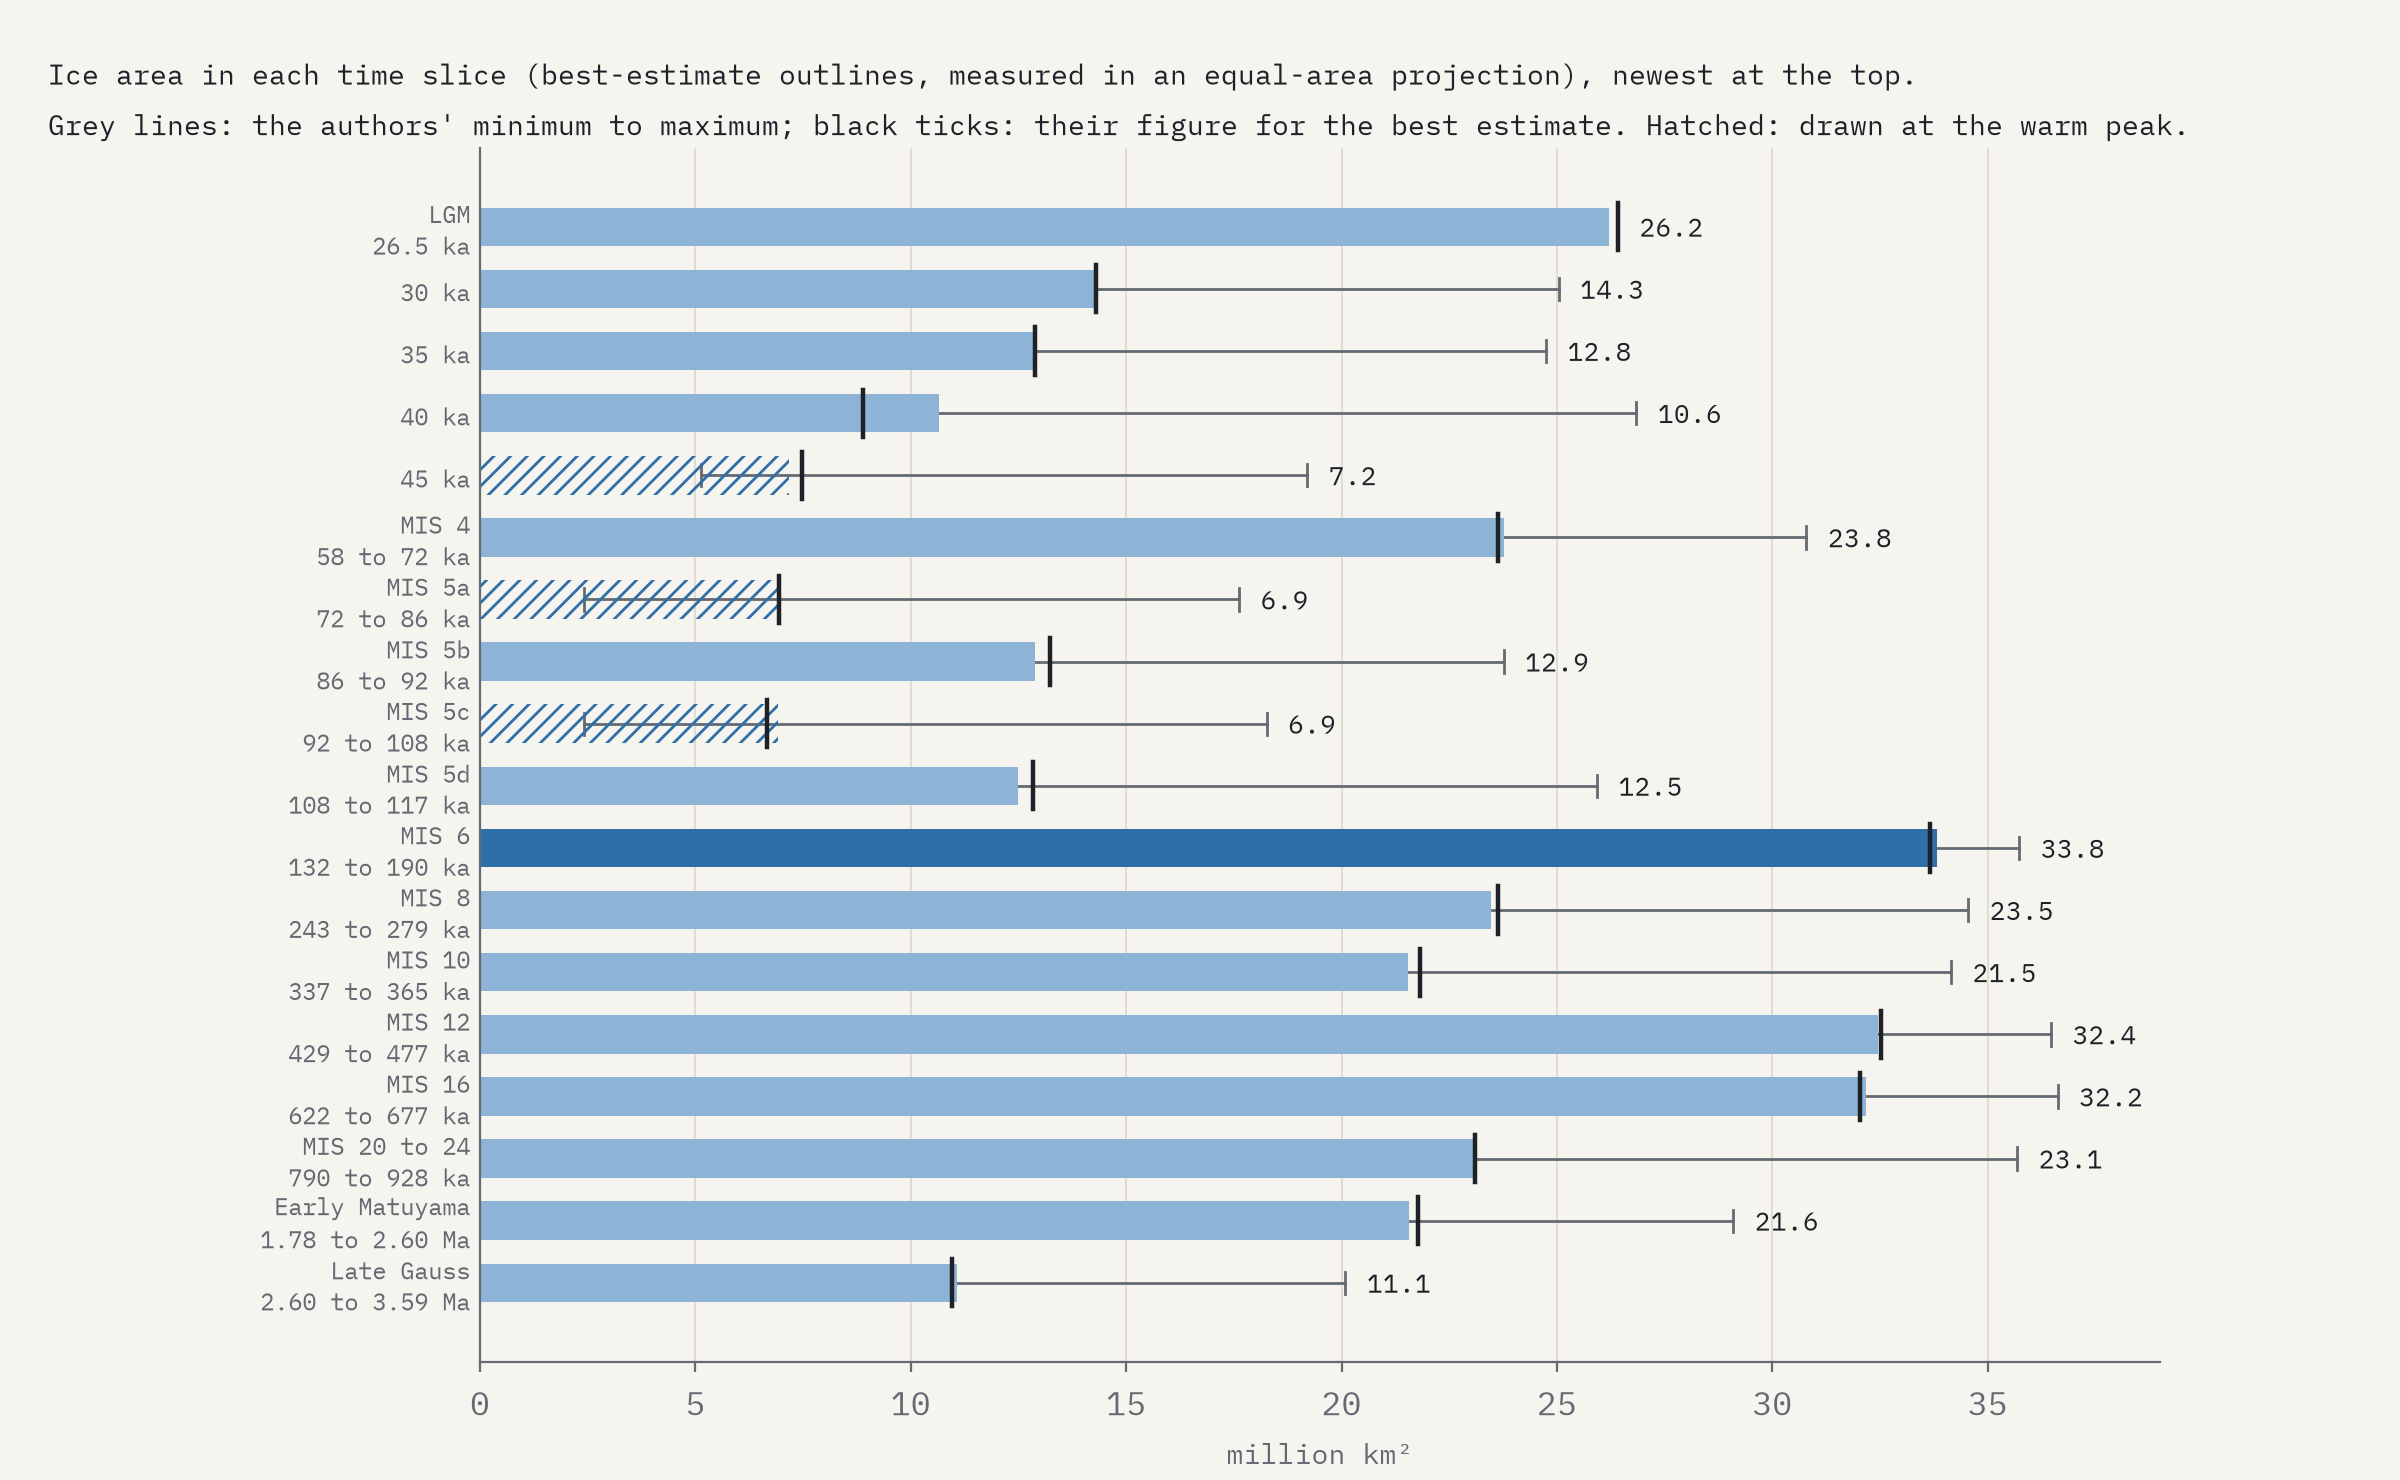
\includegraphics[width=\textwidth]{f_areas.png}
\caption{Ice area in each time slice: best-estimate outlines measured in an equal-area projection (bars), the authors' best-estimate figure (ticks) and their minimum to maximum range (lines). Hatched: slices drawn at peak warmth.}\label{fig:areas}\end{figure}

\begin{figure}[tbp]\centering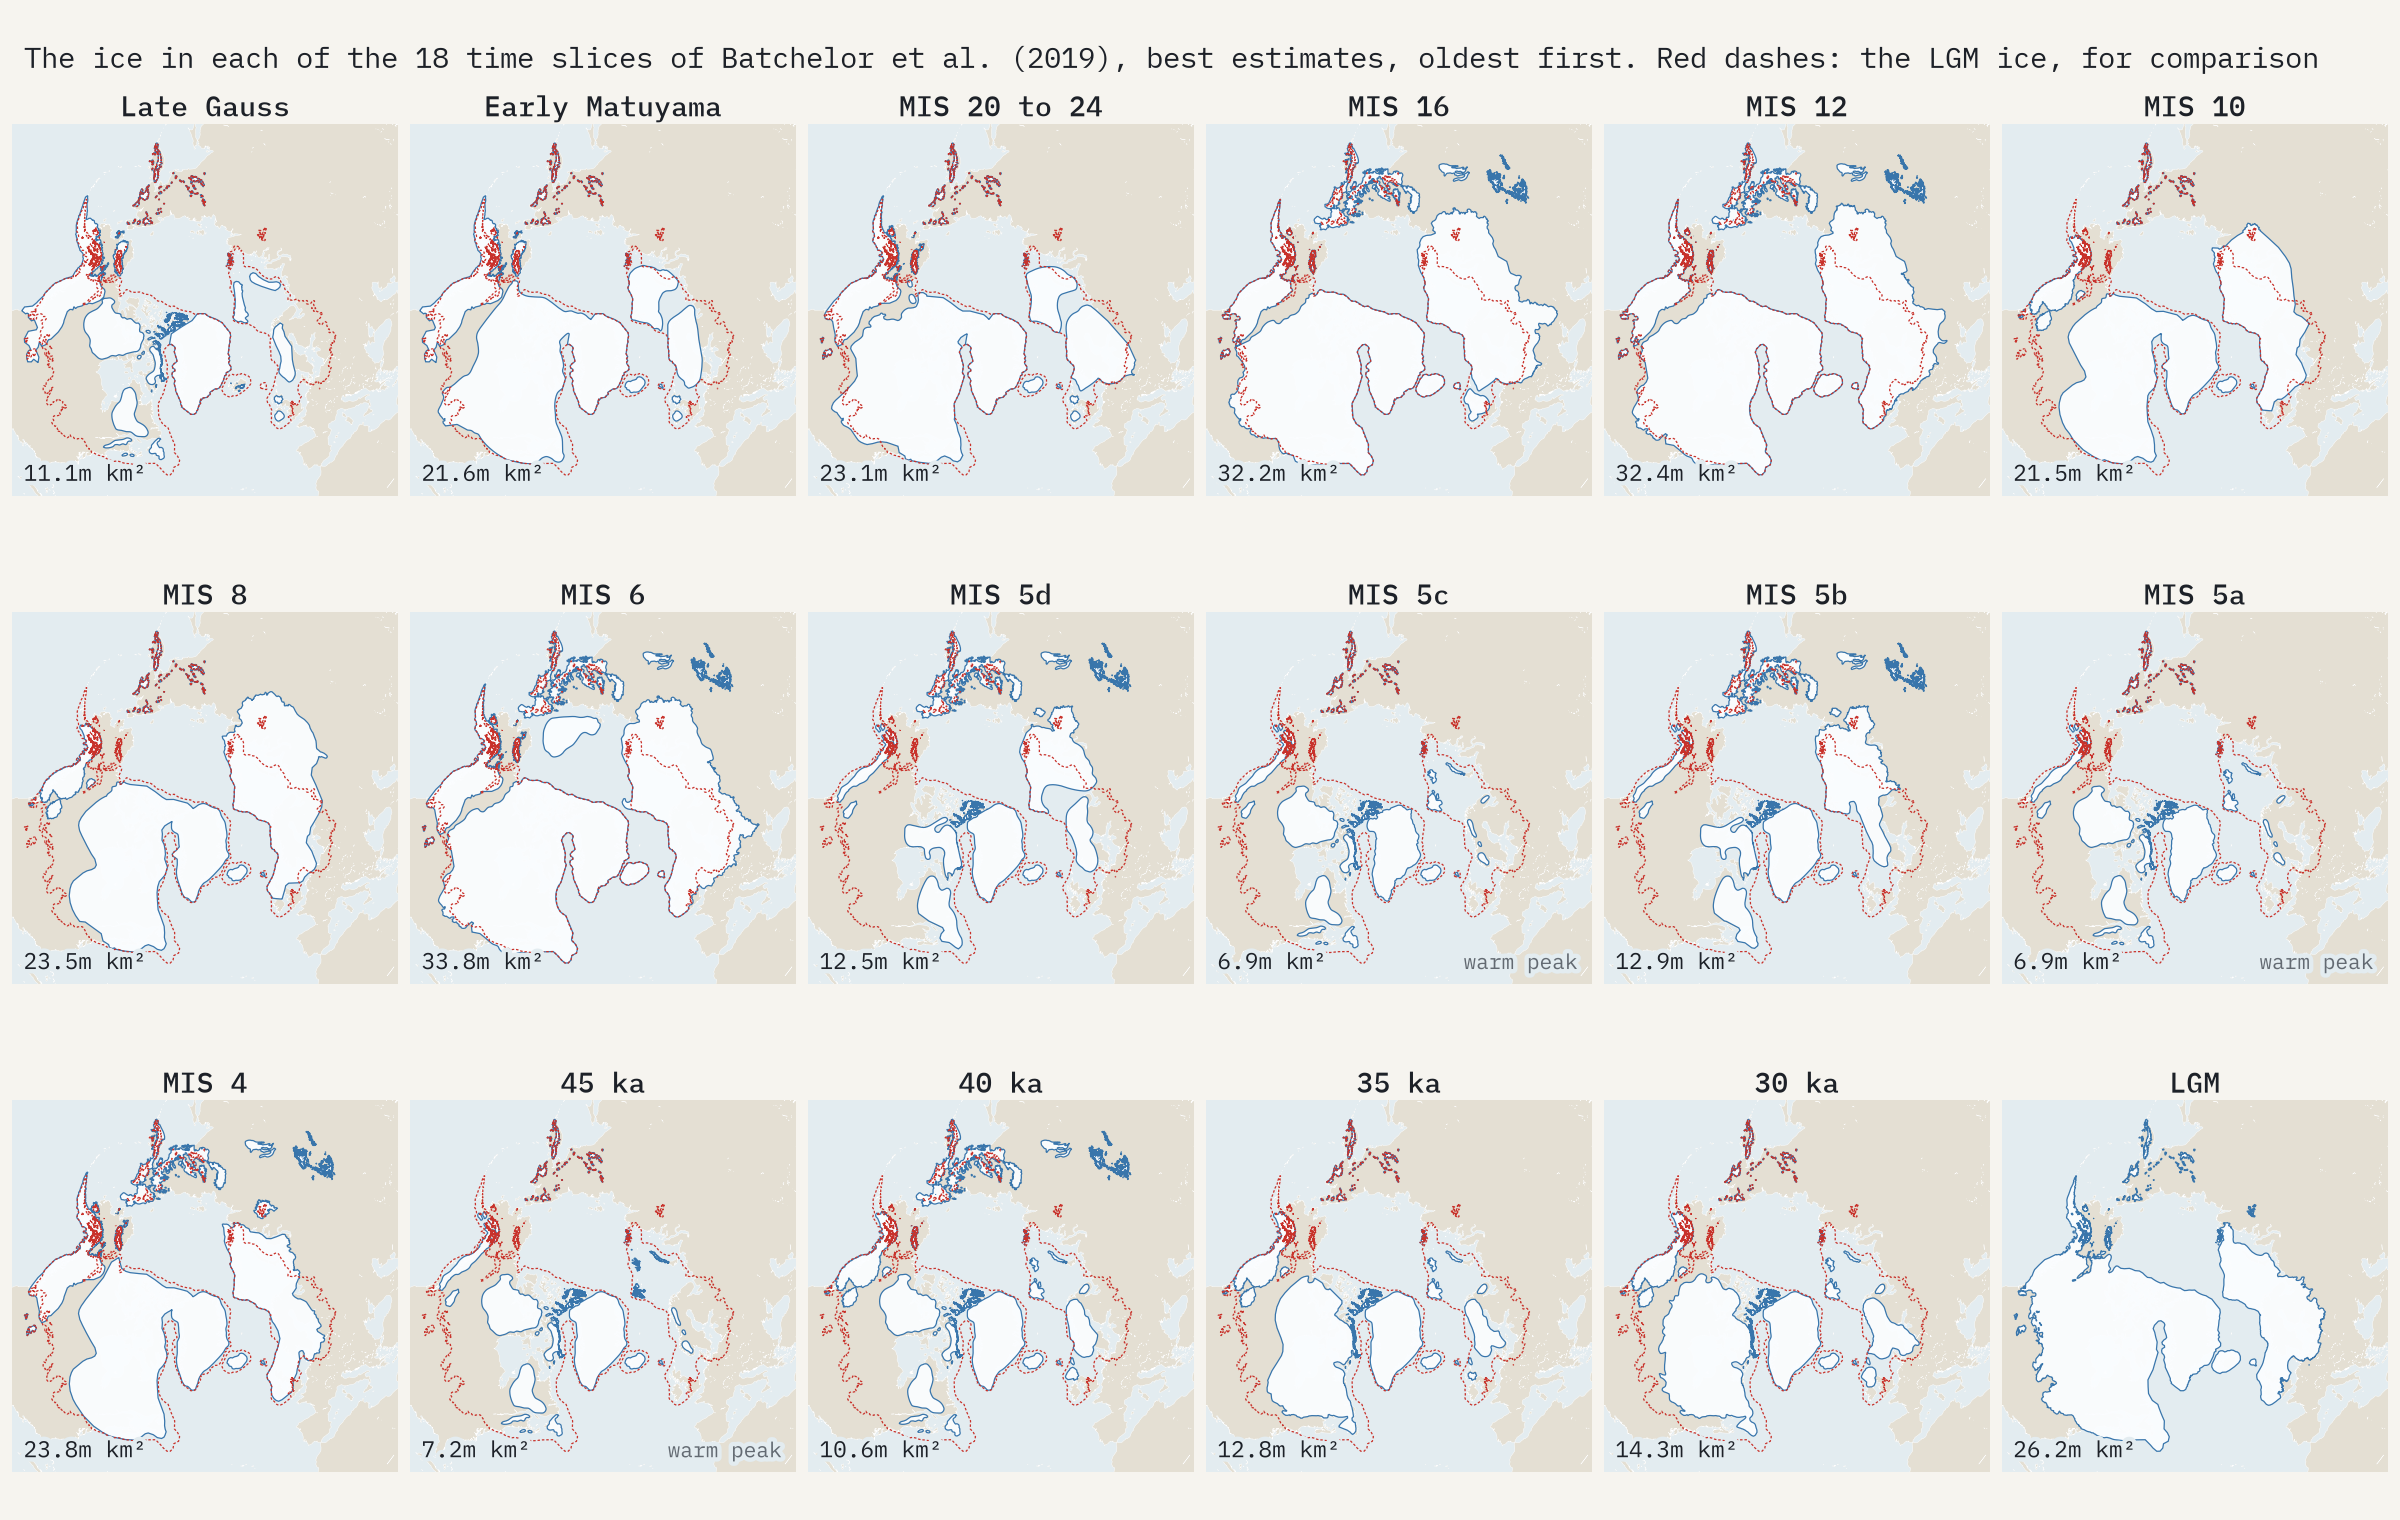
\includegraphics[width=\textwidth]{f_stages.png}
\caption{The best-estimate ice of every mapped slice, oldest first, with the LGM ice (red dashes) for comparison. North polar Lambert azimuthal equal-area projection, central meridian 40°W.}\label{fig:stages}\end{figure}

\begin{figure}[tbp]\centering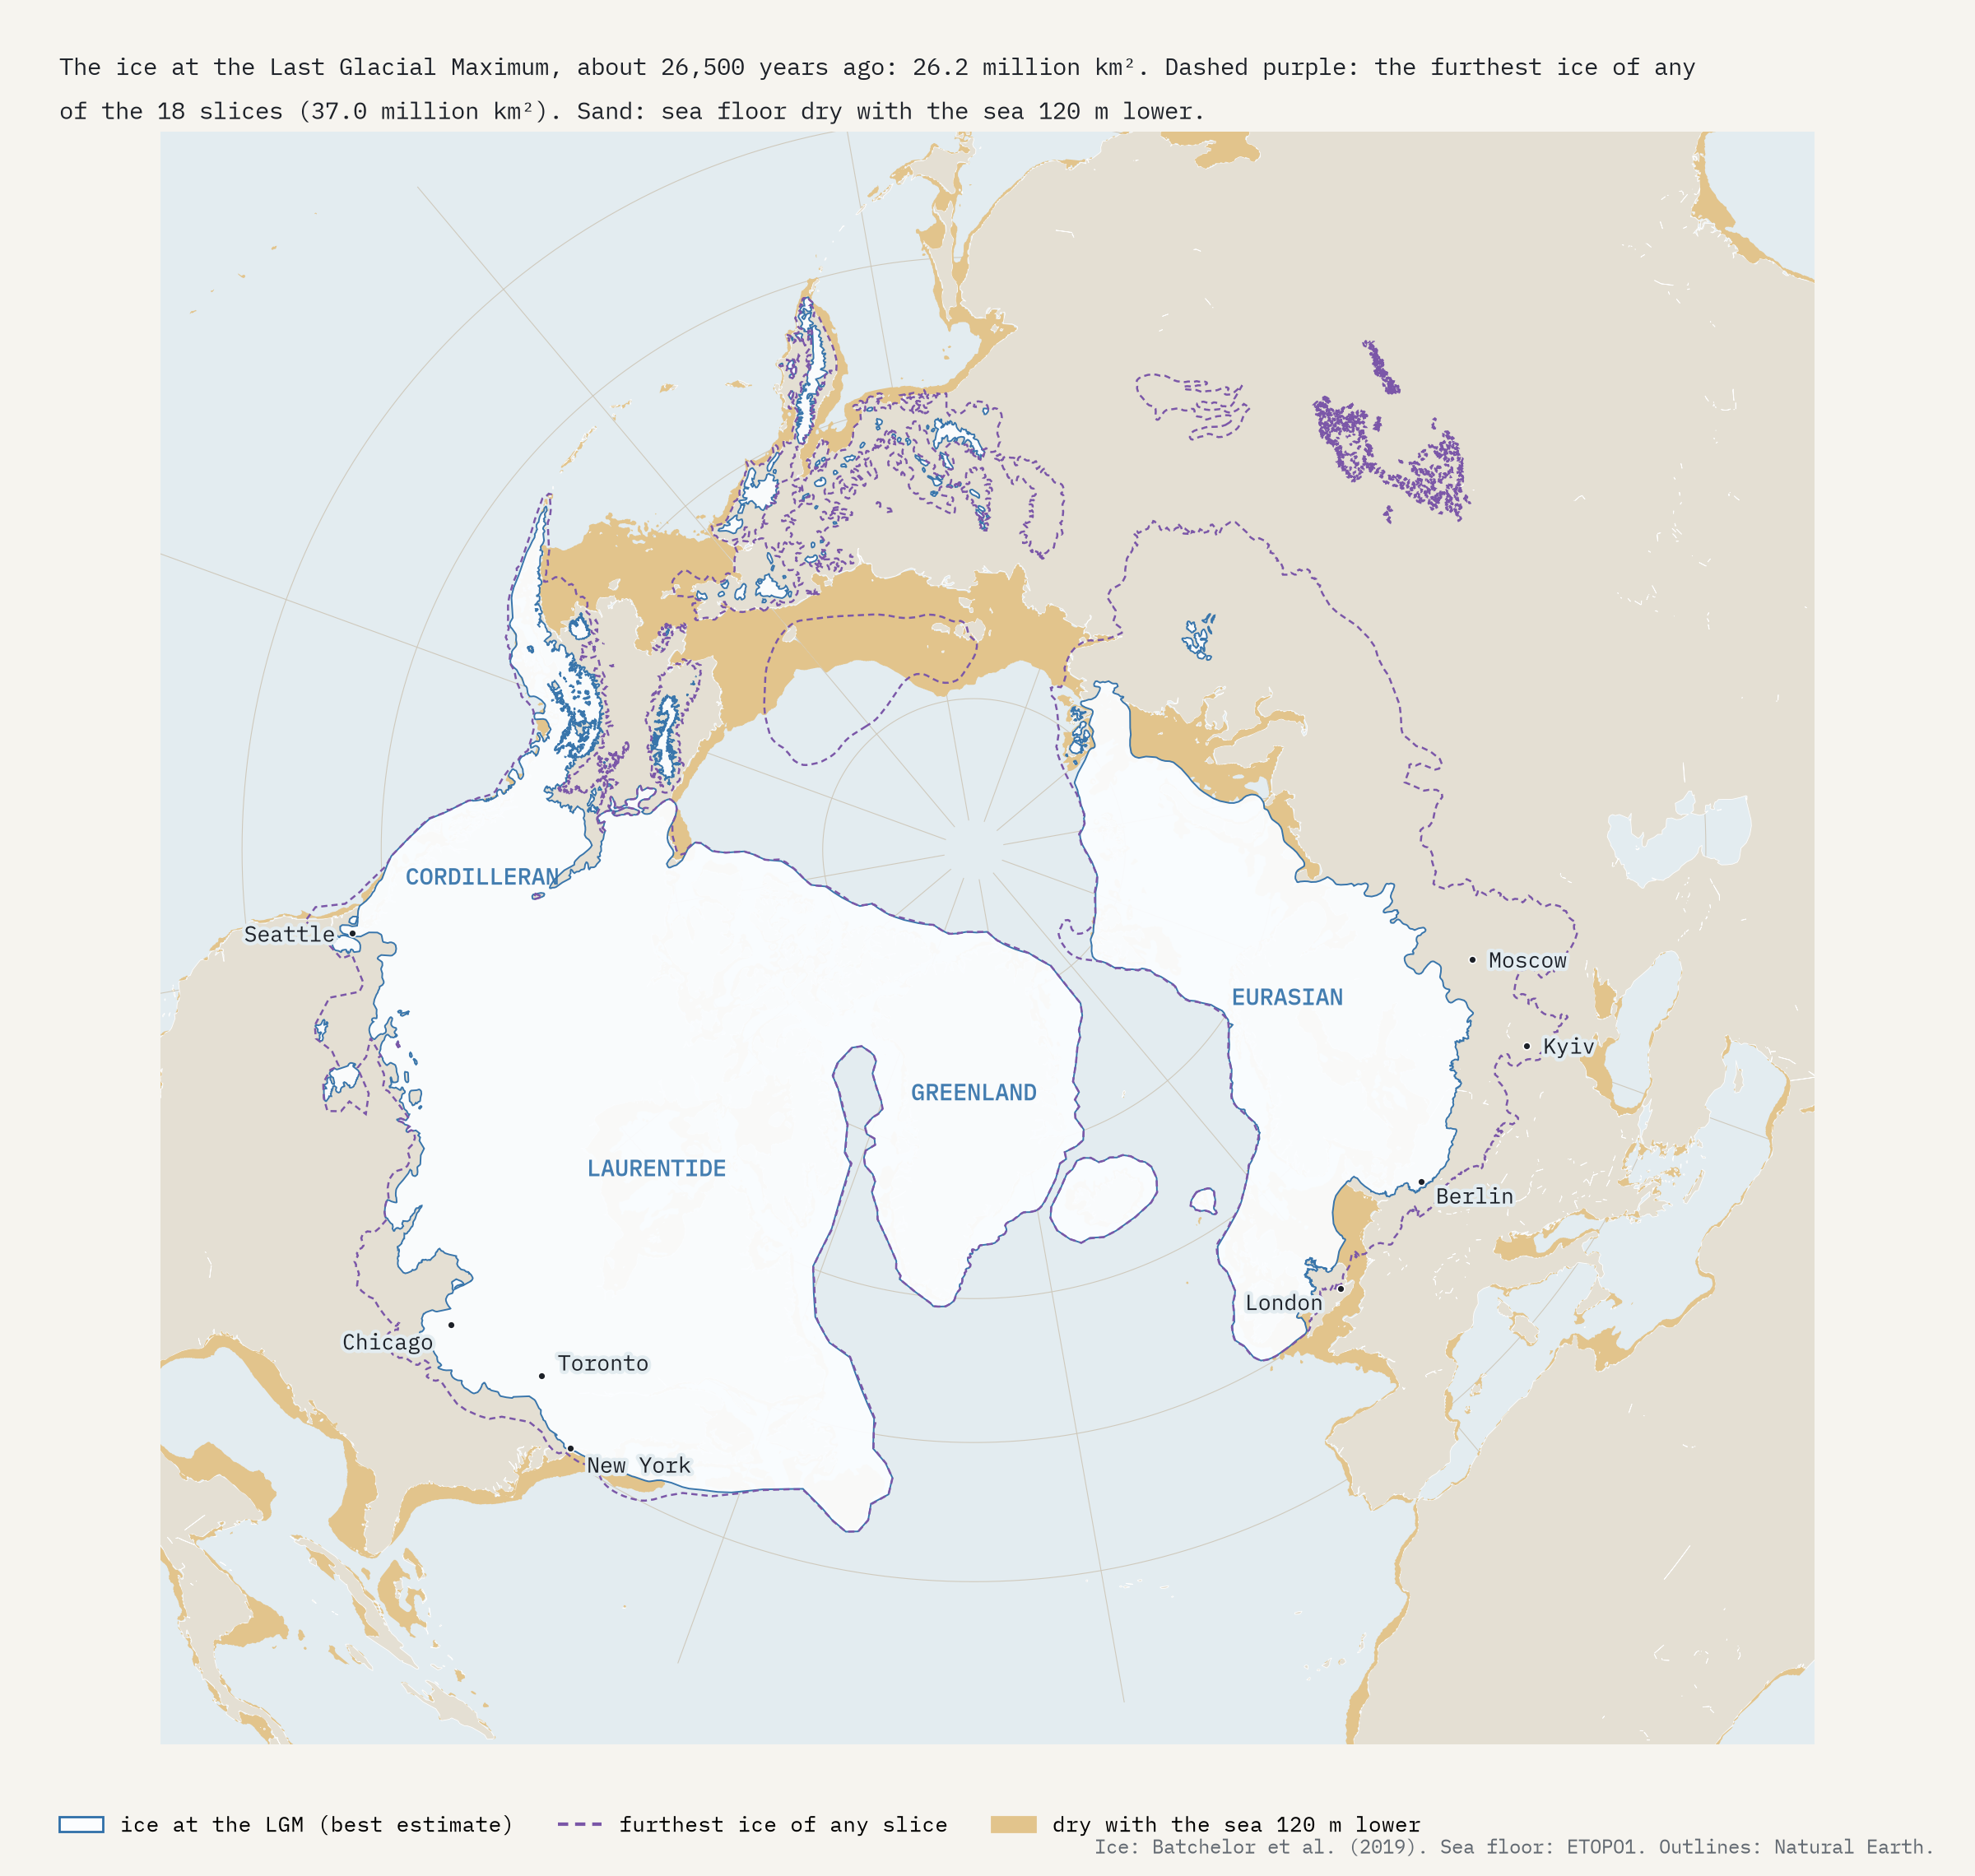
\includegraphics[width=.92\textwidth]{f_map.png}
\caption{The LGM ice, the furthest ice of any slice (dashed purple) and the sea floor exposed by a 120 m fall in sea level (sand), with selected cities.}\label{fig:map}\end{figure}

\subsection{Southernmost reach}
In North America the LGM ice reached 39.0°N, 55 km from Bloomington, Indiana. MIS 6 and MIS 12 reached 37.2°N in southern Illinois, 26 km from the confluence of the Ohio and the Mississippi. In Europe the LGM outline reaches its lowest latitude, 50.2°N, on the floor of the Celtic Sea south of Ireland; on the mainland it reaches 51.8°N. In MIS 6 a lobe reached 48.3°N in the Dnieper valley, 59 km from Dnipro, the southernmost European ice of any slice, and in MIS 16 the ice reached 48.9°N in the Don basin (Figure~\ref{fig:south}, Table~\ref{tab:south}).

\begin{table}[tbp]\centering\footnotesize\setlength{\tabcolsep}{4pt}\caption{Southernmost latitude (°N) of outline polygons of 50,000 \kmq\ or more, and the nearest Natural Earth place of 50,000 people or more.}\label{tab:south}\begin{tabular}{lrlrl}\toprule Slice & \multicolumn{2}{c}{North America} & \multicolumn{2}{c}{Europe}\\\midrule
LGM & 39.02 & Bloomington (55 km) & 50.23 & Cork (194 km)\\
30 ka & 43.49 & Rochester (47 km) & 53.16 & Grudziądz (36 km)\\
35 ka & 43.49 & Rochester (47 km) & 56.58 & Växjö (37 km)\\
40 ka & 43.48 & Manchester (78 km) & 55.75 & Glasgow (15 km)\\
45 ka & 43.48 & Manchester (78 km) & 58.71 & Kristiansand (64 km)\\
MIS 4 & 41.31 & New Bedford (39 km) & 51.29 & Cork (68 km)\\
MIS 5a & 43.48 & Manchester (78 km) & 58.71 & Kristiansand (65 km)\\
MIS 5b & 46.36 & St. John's (164 km) & 58.27 & Kristiansand (16 km)\\
MIS 5c & 43.48 & Manchester (78 km) & 58.72 & Kristiansand (64 km)\\
MIS 5d & 46.23 & St. John's (152 km) & 57.01 & Kristiansand (133 km)\\
MIS 6 & 37.22 & Evansville (158 km) & 48.30 & Dnipro (59 km)\\
MIS 8 & 41.46 & New Bedford (184 km) & 54.00 & Rostock (40 km)\\
MIS 10 & 41.16 & New Bedford (229 km) & 54.00 & Rostock (38 km)\\
MIS 12 & 37.22 & Evansville (158 km) & 49.27 & Drohobych (12 km)\\
MIS 16 & 37.82 & Belleville (97 km) & 48.86 & Kamensk Shakhtinskiy (147 km)\\
MIS 20 to 24 & 38.06 & Belleville (79 km) & 49.72 & Ostrava (34 km)\\
Early Matuyama & 37.92 & Belleville (117 km) & 52.18 & Cork (64 km)\\
Late Gauss & 42.52 & Casper (144 km) & 52.18 & Cork (64 km)\\
\bottomrule\end{tabular}\end{table}

\begin{figure}[tbp]\centering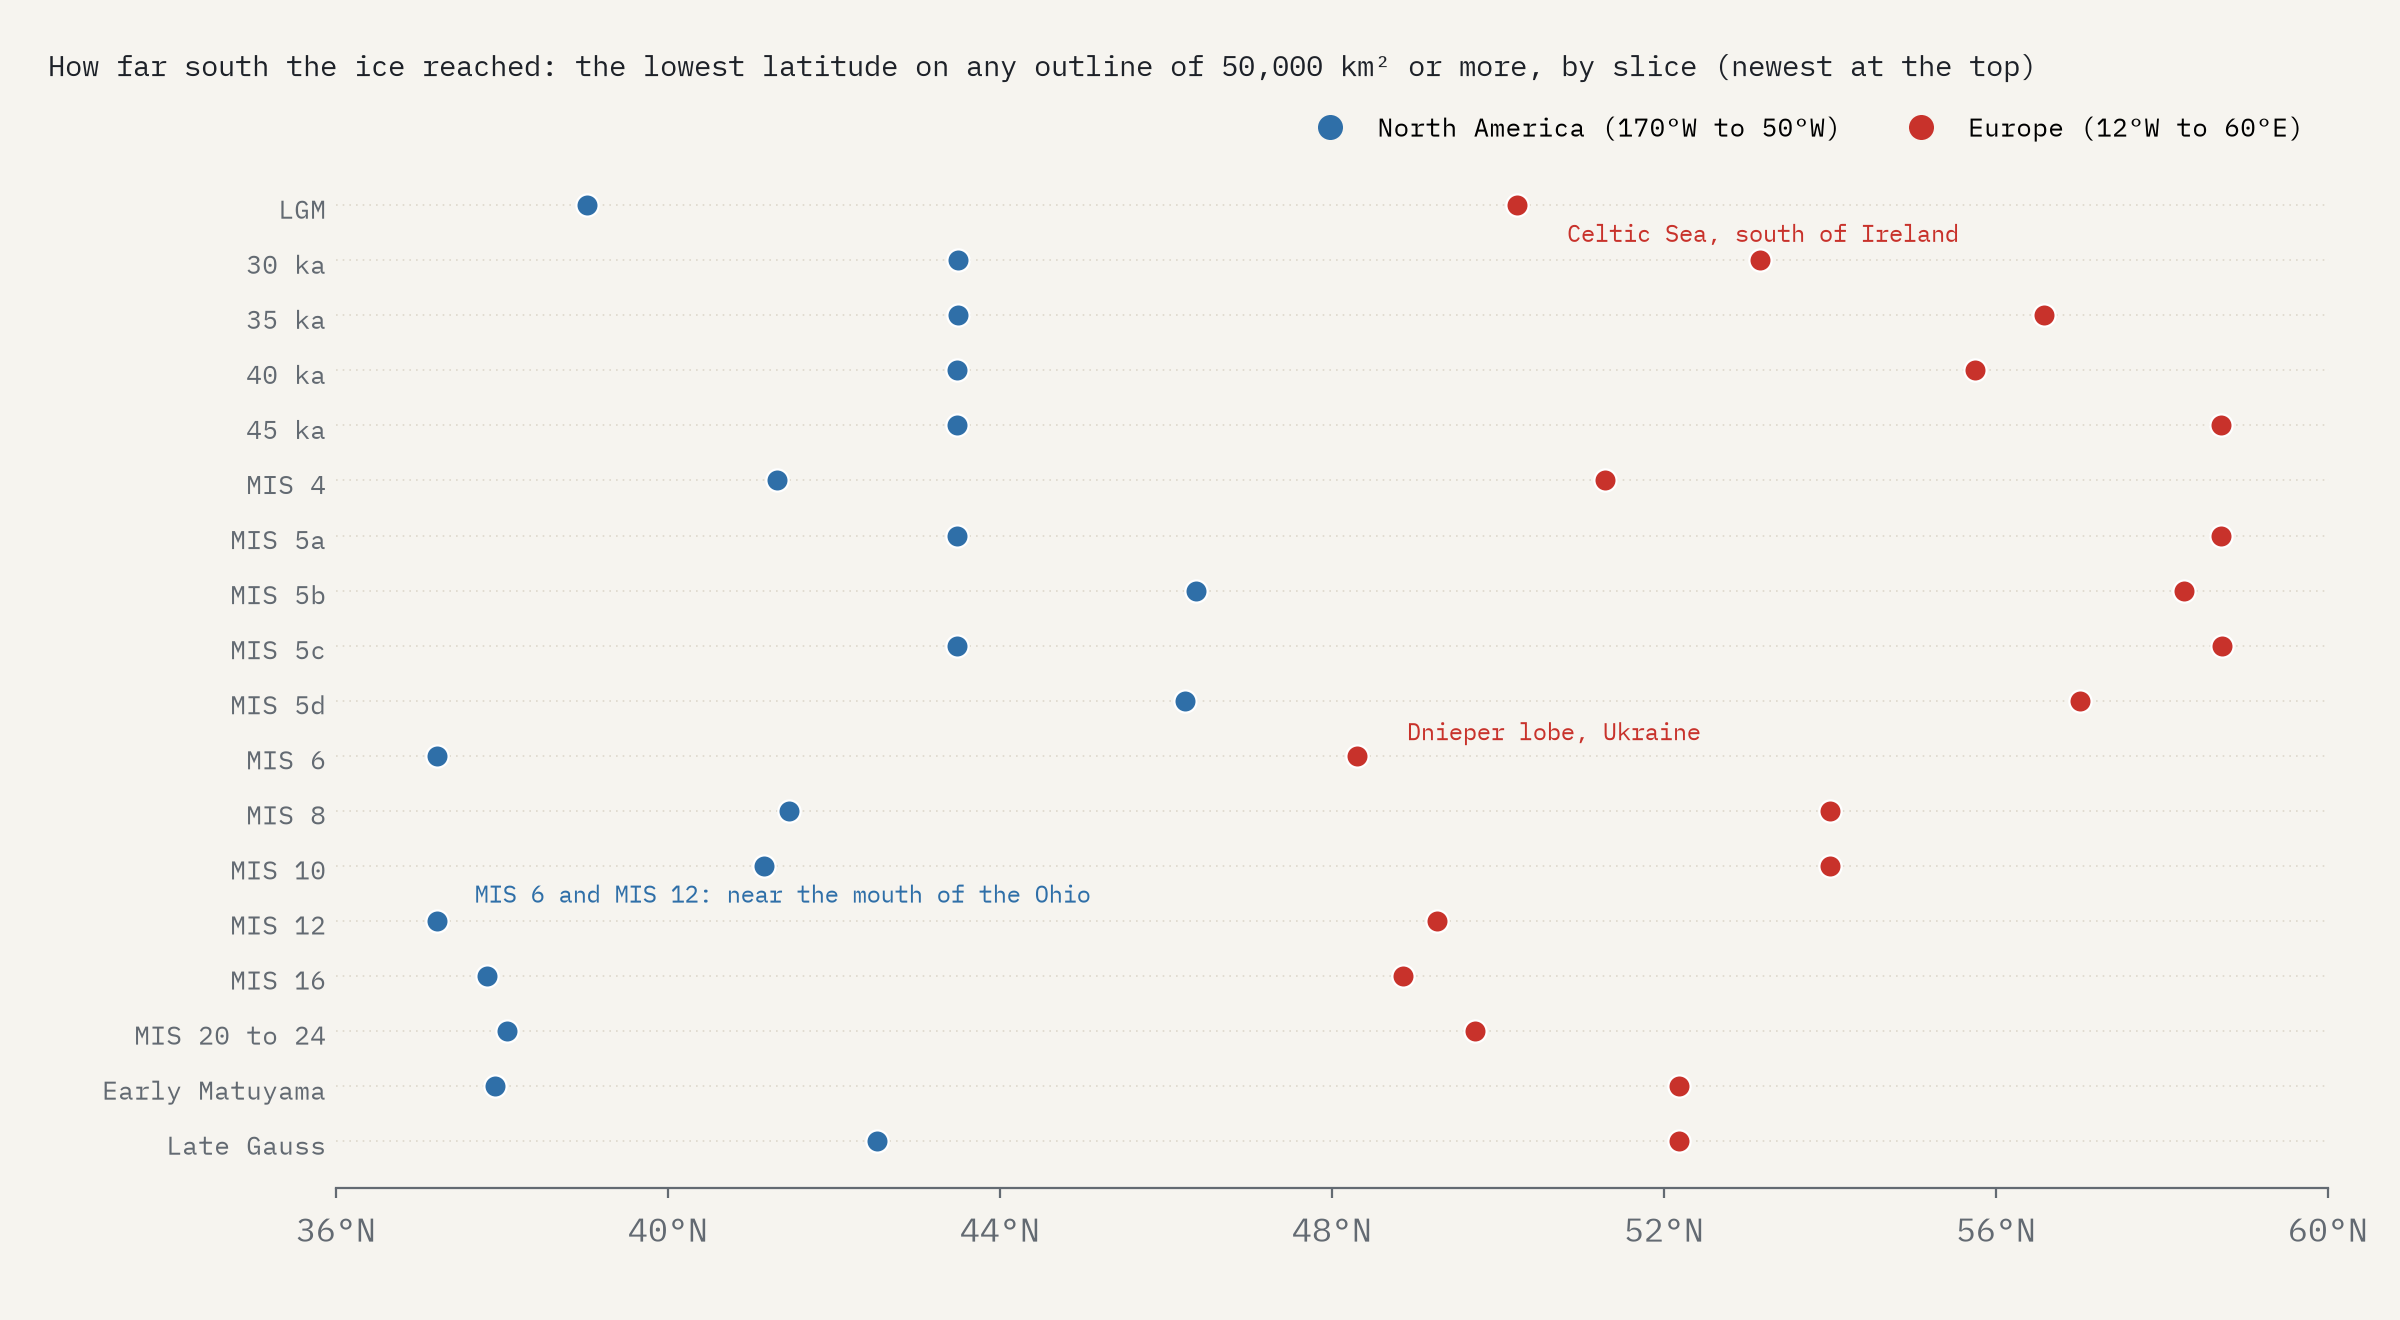
\includegraphics[width=\textwidth]{f_south.png}
\caption{Lowest latitude of the ice in North America and Europe in each slice (outline polygons of 50,000 \kmq\ or more).}\label{fig:south}\end{figure}

\subsection{What lay beneath}
The LGM outline covers at least 1\% of 21 countries and territories, and the union of all outlines 25. Under the LGM ice were 97.4\% of Canada, all of Ireland, Sweden, Finland, Iceland, Estonia and Latvia, 99.9\% of Norway, 96.3\% of Lithuania, 75.1\% of Denmark, 60.9\% of the United Kingdom, 37.6\% of Poland, 21.2\% of the United States, 13.5\% of Germany and 7.1\% of Russia. Across all slices the shares rise to 94.7\% for Poland, 97.6\% for Belarus, 60.2\% for the Netherlands, 46.8\% for Germany, 43.1\% for Russia and 28.2\% for Ukraine (Figure~\ref{fig:countries}).

709 Natural Earth places lie inside the LGM outline, 27 of them with a population figure of a million or more; their figures sum to 140,570,036, 5.9\% of the sum for all places. The union of all outlines contains 1,050 places summing to 230,083,190. Table~\ref{tab:cities} gives distances to the LGM edge for the cities chosen in advance (Figure~\ref{fig:cities}). New York is 13 km inside the LGM outline, consistent with the usual account that the ice reached Manhattan \citep{wiki}; Chicago is 112 km inside, Berlin 42 km and Seattle 17 km. London is outside every outline, 152 km from the LGM edge and 16 km from that of MIS 12, the Anglian glaciation; Moscow is 246 km outside the LGM ice but inside three older outlines. Given the generalisation of the outlines, distances under a few tens of kilometres say only that a city was near the edge.

\begin{table}[tbp]\centering\scriptsize\setlength{\tabcolsep}{3pt}\caption{Distance from city centres to the LGM ice edge (km; negative inside the ice) and the slices whose best-estimate outline contains the city.}\label{tab:cities}\begin{tabular}{llrrp{7.2cm}}\toprule City & Country & km & Slices & Which\\\midrule
Stockholm & Sweden & -616 & 9 & MIS 20 to 24, MIS 16, MIS 12, MIS 10, MIS 8, MIS 6, MIS 4, 30 ka, LGM\\
Helsinki & Finland & -542 & 7 & MIS 20 to 24, MIS 16, MIS 12, MIS 8, MIS 6, MIS 4, LGM\\
Montreal & Canada & -512 & 11 & Early Matuyama, MIS 20 to 24, MIS 16, MIS 12, MIS 10, MIS 8, MIS 6, MIS 4, 35 ka, 30 ka, LGM\\
Winnipeg & Canada & -402 & 6 & Early Matuyama, MIS 20 to 24, MIS 16, MIS 12, MIS 6, LGM\\
Oslo & Norway & -401 & 14 & Early Matuyama, MIS 20 to 24, MIS 16, MIS 12, MIS 10, MIS 8, MIS 6, MIS 5d, MIS 5b, MIS 4, 40 ka, 35 ka, 30 ka, LGM\\
St Petersburg & Russia & -243 & 5 & MIS 20 to 24, MIS 16, MIS 12, MIS 6, LGM\\
Edinburgh & United Kingdom & -208 & 8 & MIS 16, MIS 12, MIS 10, MIS 8, MIS 6, MIS 4, 30 ka, LGM\\
Copenhagen & Denmark & -202 & 9 & MIS 20 to 24, MIS 16, MIS 12, MIS 10, MIS 8, MIS 6, MIS 4, 30 ka, LGM\\
Detroit & United States of America & -196 & 6 & Early Matuyama, MIS 20 to 24, MIS 16, MIS 12, MIS 6, LGM\\
Toronto & Canada & -190 & 9 & Early Matuyama, MIS 20 to 24, MIS 16, MIS 12, MIS 10, MIS 8, MIS 6, MIS 4, LGM\\
Dublin & Ireland & -180 & 5 & MIS 16, MIS 12, MIS 6, MIS 4, LGM\\
Boston & United States of America & -116 & 9 & Early Matuyama, MIS 20 to 24, MIS 16, MIS 12, MIS 10, MIS 8, MIS 6, MIS 4, LGM\\
Chicago & United States of America & -112 & 6 & Early Matuyama, MIS 20 to 24, MIS 16, MIS 12, MIS 6, LGM\\
Cleveland & United States of America & -86 & 3 & MIS 20 to 24, MIS 16, LGM\\
Calgary & Canada & -82 & 8 & Late Gauss, Early Matuyama, MIS 20 to 24, MIS 16, MIS 12, MIS 6, MIS 4, LGM\\
Vancouver & Canada & -72 & 8 & Late Gauss, Early Matuyama, MIS 20 to 24, MIS 16, MIS 12, MIS 6, MIS 4, LGM\\
Berlin & Germany & -42 & 5 & MIS 20 to 24, MIS 16, MIS 12, MIS 6, LGM\\
Minneapolis & United States of America & -28 & 6 & Early Matuyama, MIS 20 to 24, MIS 16, MIS 12, MIS 6, LGM\\
Seattle & United States of America & -17 & 8 & Late Gauss, Early Matuyama, MIS 20 to 24, MIS 16, MIS 12, MIS 6, MIS 4, LGM\\
New York & United States of America & -13 & 4 & MIS 16, MIS 12, MIS 6, LGM\\
Manchester & United Kingdom & -10 & 5 & MIS 16, MIS 12, MIS 6, MIS 4, LGM\\
Hamburg & Germany & 12 & 2 & MIS 12, MIS 6\\
Cincinnati & United States of America & 16 & 4 & MIS 20 to 24, MIS 16, MIS 12, MIS 6\\
Warsaw & Poland & 80 & 4 & MIS 20 to 24, MIS 16, MIS 12, MIS 6\\
Philadelphia & United States of America & 82 & 1 & MIS 16\\
Minsk & Belarus & 91 & 3 & MIS 16, MIS 12, MIS 6\\
St Louis & United States of America & 151 & 1 & MIS 20 to 24\\
London & United Kingdom & 152 & 0 & none\\
Amsterdam & Netherlands & 183 & 1 & MIS 6\\
Prague & Czechia & 200 & 0 & none\\
Moscow & Russia & 246 & 3 & MIS 16, MIS 12, MIS 6\\
Krakow & Poland & 256 & 1 & MIS 16\\
Kansas City & United States of America & 275 & 1 & MIS 20 to 24\\
Kyiv & Ukraine & 456 & 1 & MIS 6\\
Paris & France & 464 & 0 & none\\
\bottomrule\end{tabular}\end{table}

\begin{figure}[tbp]\centering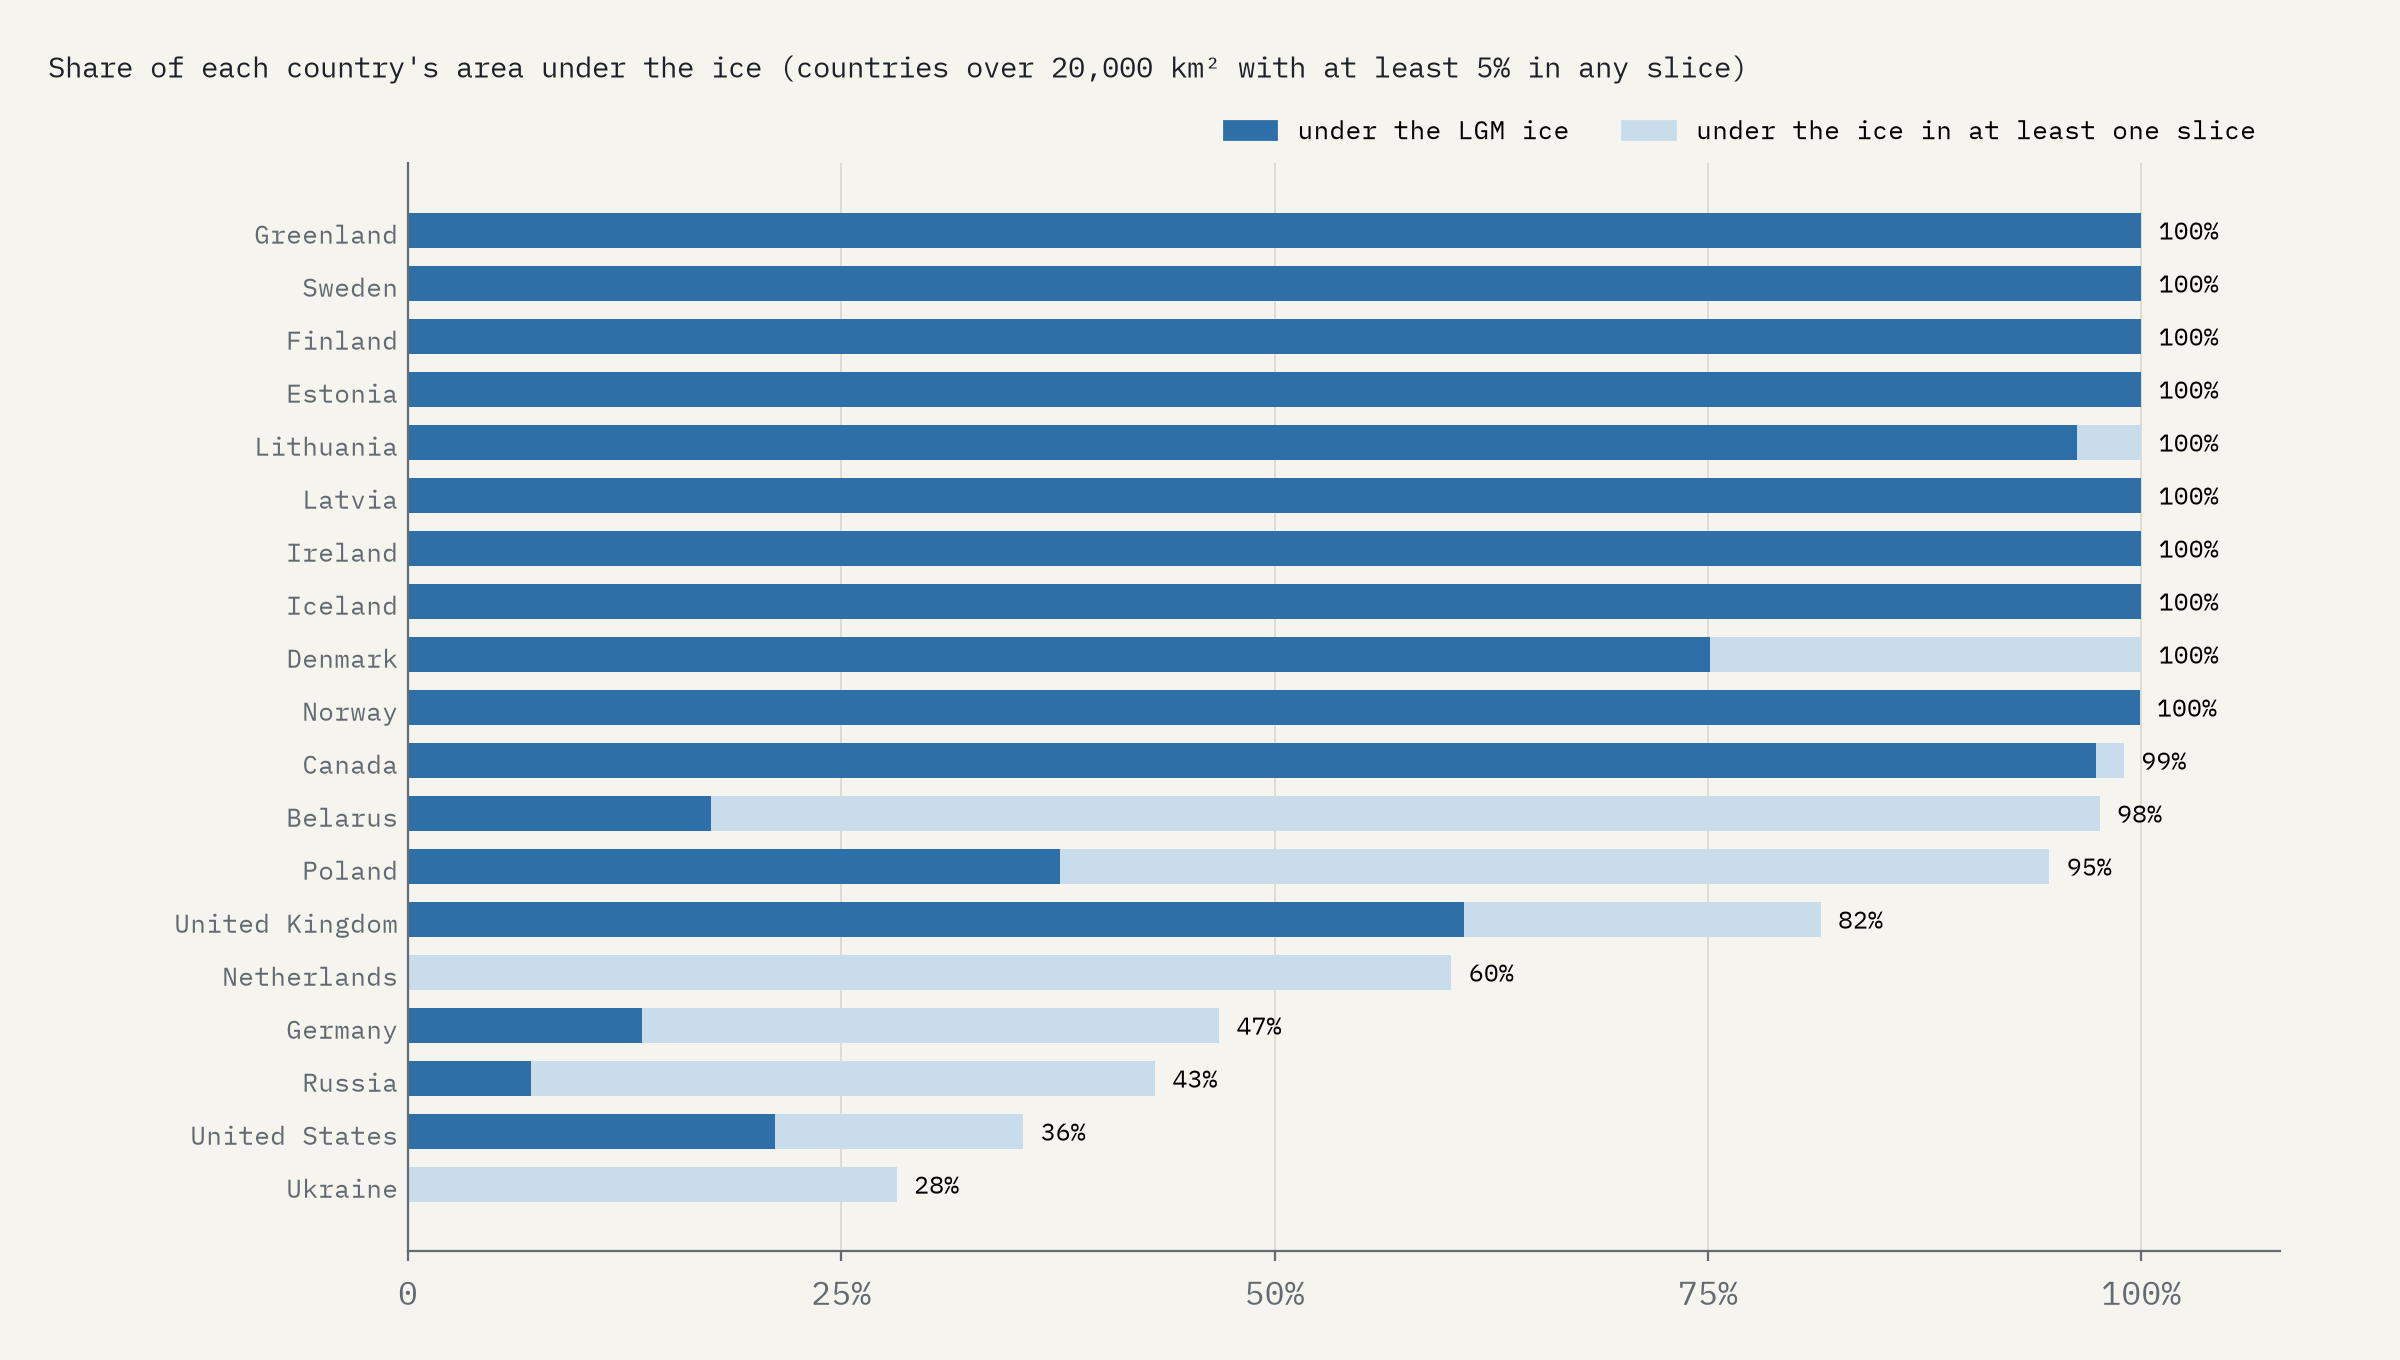
\includegraphics[width=\textwidth]{f_countries.png}
\caption{Share of each country under the LGM ice and under the ice of at least one slice.}\label{fig:countries}\end{figure}

\begin{figure}[tbp]\centering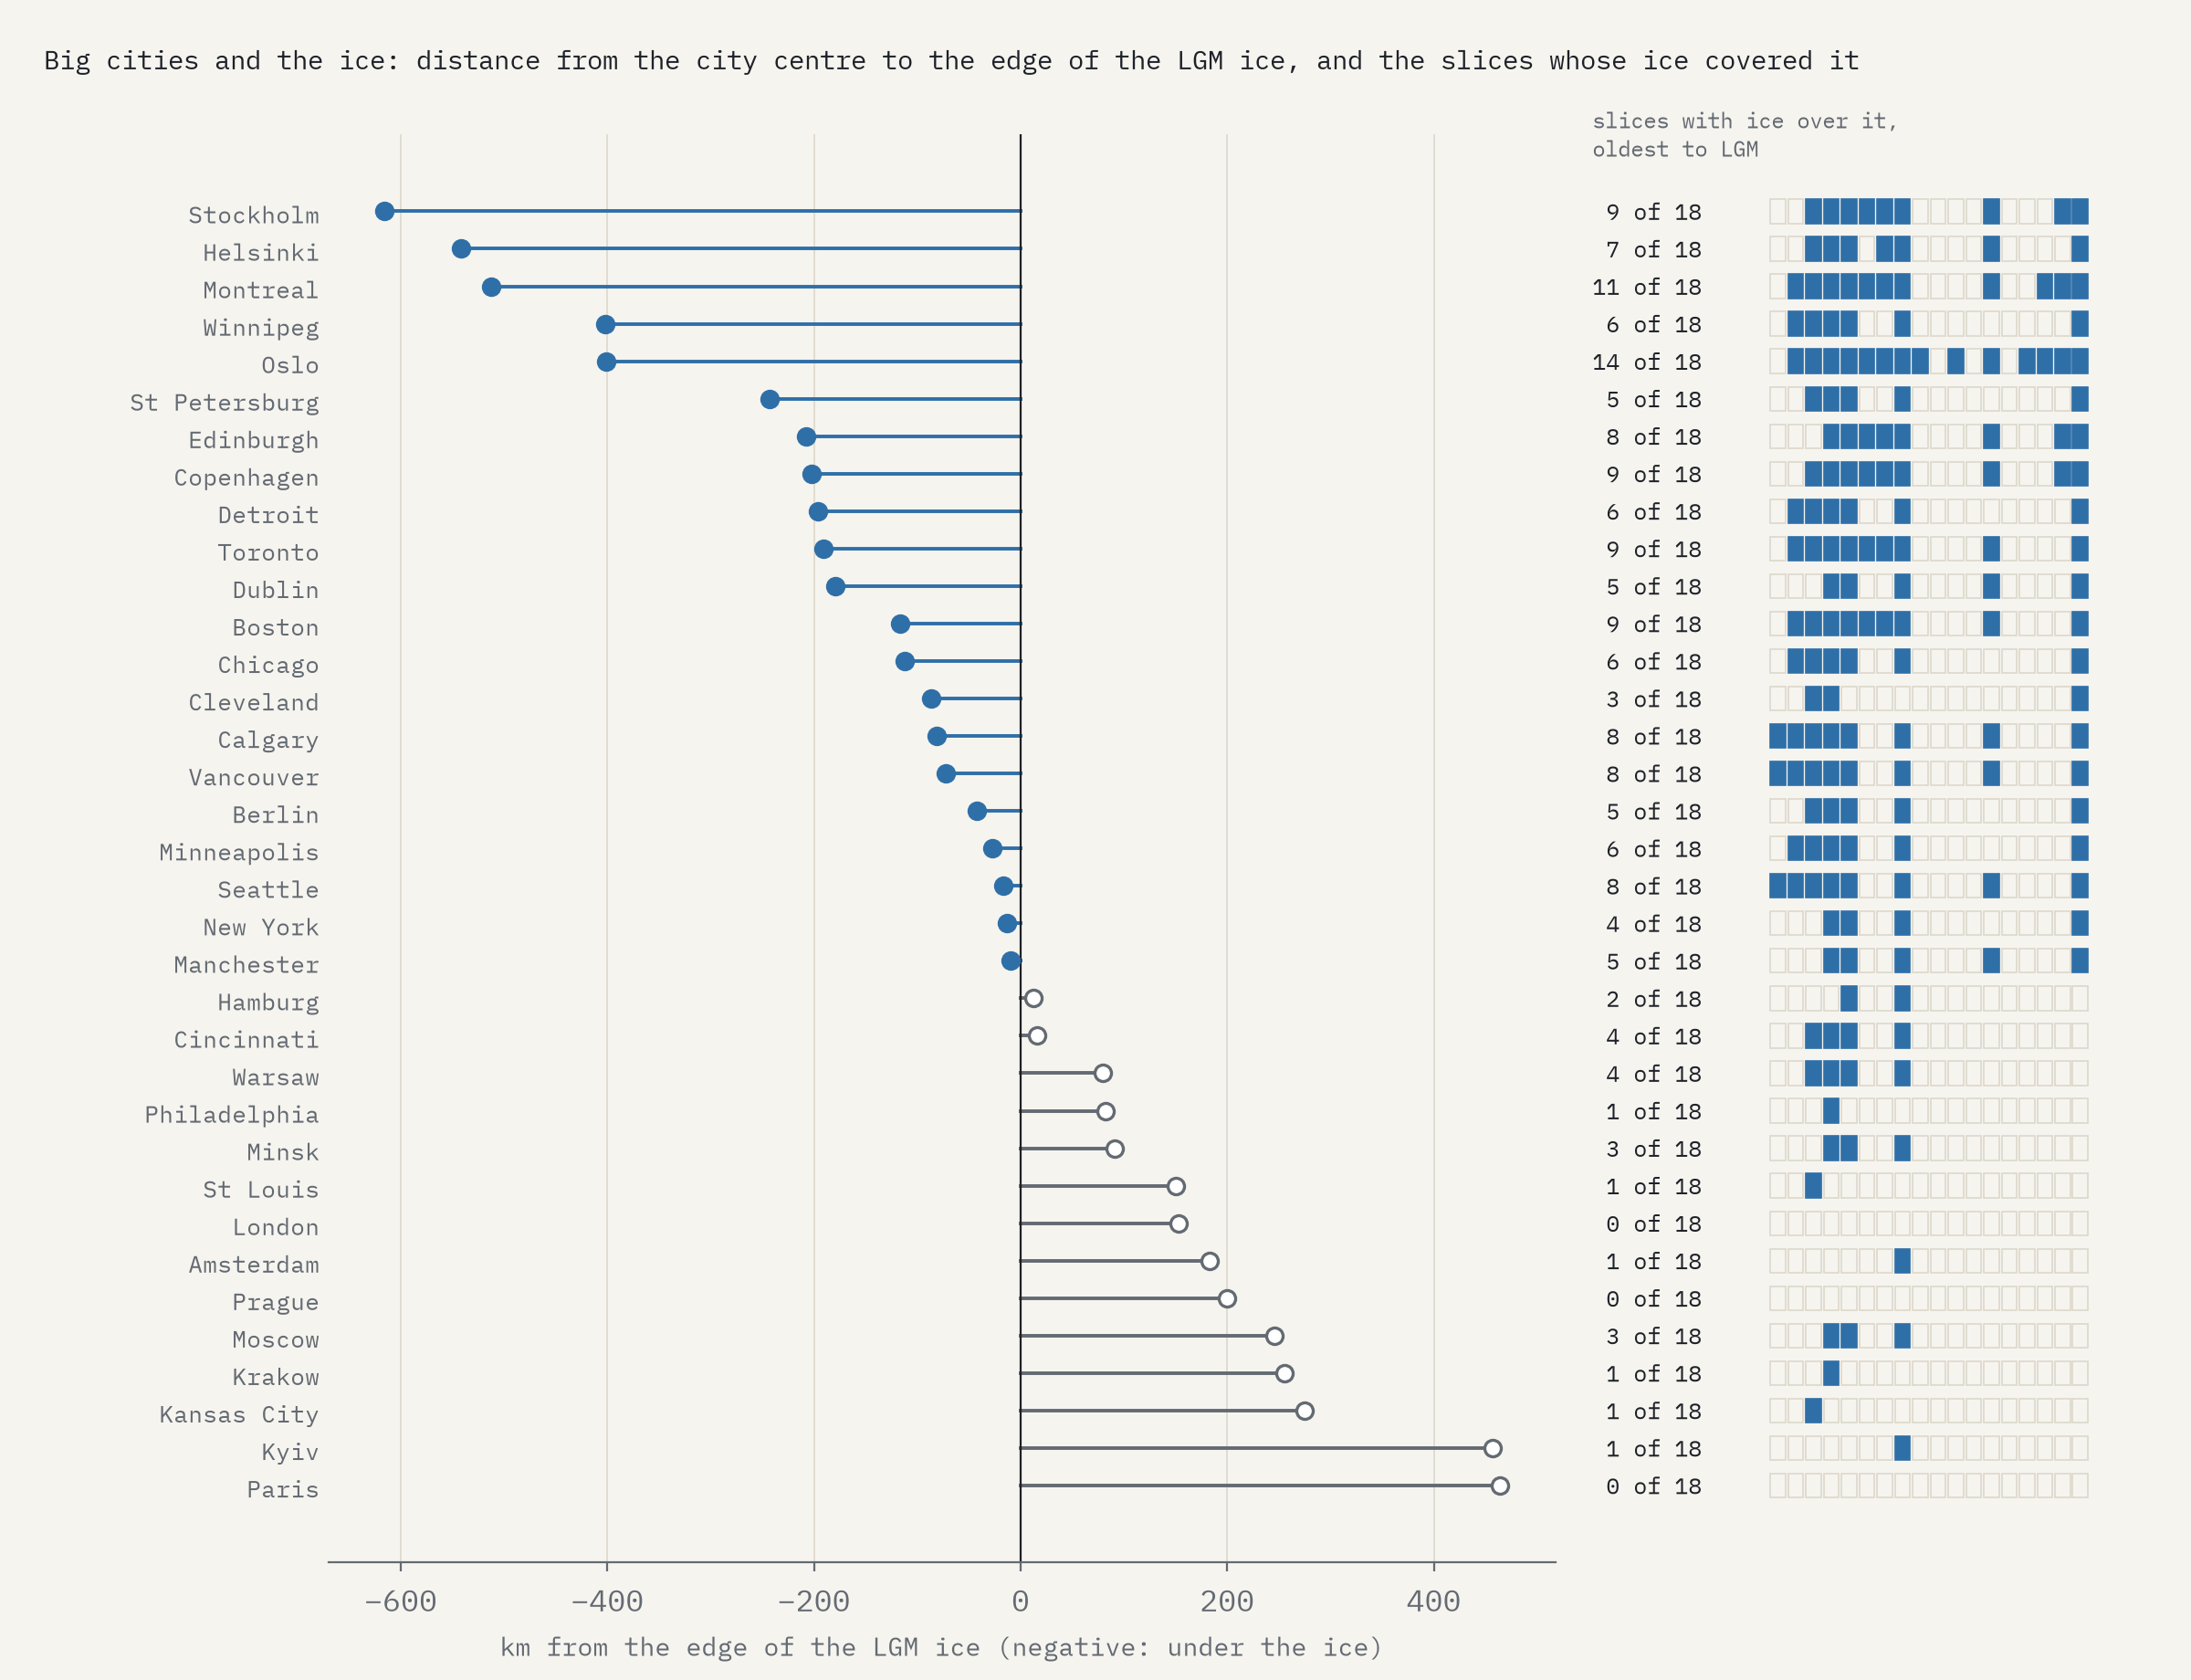
\includegraphics[width=\textwidth]{f_cities.png}
\caption{Distance from city centres to the LGM ice edge (negative inside), and the slices whose outline contains each city, oldest on the left.}\label{fig:cities}\end{figure}

\subsection{Exposed sea floor}
A sea level 120 m below today's exposes 21,174,383 \kmq\ of sea floor on the ETOPO10 grid, 14.2\% of today's land area of 148,753,862 \kmq. Of this, 3,699,394 \kmq\ lies inside the LGM ice outline, leaving 17,474,989 \kmq\ of ice-free new land. A 60 m fall exposes 14,257,424 \kmq, 67\% of the 120 m figure. By region (Table~\ref{tab:shelves}, Figure~\ref{fig:exposed}) the largest ice-free gains at 120 m are the Sahul shelf (2,859,872 \kmq), the Sunda shelf (2,345,574), the Laptev, Kara and East Siberian shelves (1,810,593) and Beringia (1,641,739). The boxes hold 64\% of all ice-free exposed floor. Along the meridian of the Bering Strait (168.75°W), land and exposed floor run without a break for 1,914 km, from 56.4°N to 73.6°N. All 11 land-bridge tests (Britain and Europe, Ireland and Britain, Asia and North America, New Guinea and Tasmania with Australia, Sumatra, Java and Borneo with mainland Asia, Sri Lanka with India, Taiwan and Sakhalin with the mainland) are joined at 60 m as well as at 120 m, and none at today's level.

\begin{table}[tbp]\centering\scriptsize\setlength{\tabcolsep}{3pt}\caption{Sea floor exposed by sea levels 60 m and 120 m below today's in the shelf boxes (\kmq): ice-free at 60 m and 120 m, and all exposed floor at 120 m including that under the LGM ice. Boxes: Sahul 112..155°E, $-$45..$-$2°N; Sundaland 95..120°E, $-$9..14°N; Siberian Arctic shelf 55..180°E, 66..82°N; Beringia $-$180..$-$155°E, 52..75°N; 160..180°E, 52..72°N; East China and Yellow seas 117..131°E, 22..41°N; Patagonian shelf $-$70..$-$52°E, $-$56..$-$35°N; Doggerland $-$12..10°E, 48..62°N; Persian Gulf 47..57°E, 23..31°N; Grand Banks and New England $-$75..$-$45°E, 38..52°N; Barents Sea 10..55°E, 66..82°N; Canadian Arctic and Hudson Bay $-$125..$-$60°E, 50..84°N.}\label{tab:shelves}\begin{tabular}{lp{5.6cm}rrr}\toprule Region & Seas & 60 m & 120 m & 120 m, all\\\midrule
Sahul & Sahul and Arafura shelves, Gulf of Carpentaria, Bass Strait & 2,169,476 & 2,859,872 & 2,859,872\\
Sundaland & Sunda Shelf: Gulf of Thailand, Java Sea, southern South China Sea & 1,767,483 & 2,345,574 & 2,345,574\\
Siberian Arctic shelf & Laptev, East Siberian and Kara seas & 1,537,425 & 1,810,593 & 2,034,737\\
Beringia & Bering and Chukchi seas & 1,186,711 & 1,641,739 & 1,713,742\\
East China and Yellow seas & Yellow Sea, Bohai, East China Sea, Taiwan Strait & 587,773 & 1,018,450 & 1,018,450\\
Patagonian shelf & Argentine shelf and the Falklands & 262,245 & 784,516 & 784,516\\
Doggerland & North Sea, English Channel and the Irish Sea & 213,192 & 277,636 & 787,162\\
Persian Gulf & the whole Gulf & 202,492 & 250,154 & 250,154\\
Grand Banks and New England & Gulf of Maine, Scotian Shelf, Grand Banks & 60,971 & 108,288 & 606,542\\
Barents Sea & Barents and White seas & 38,748 & 39,695 & 413,572\\
Canadian Arctic and Hudson Bay & Canadian Arctic Archipelago, Hudson Bay, Baffin Bay shelves & 0 & 0 & 1,181,934\\
\bottomrule\end{tabular}\end{table}

\begin{figure}[tbp]\centering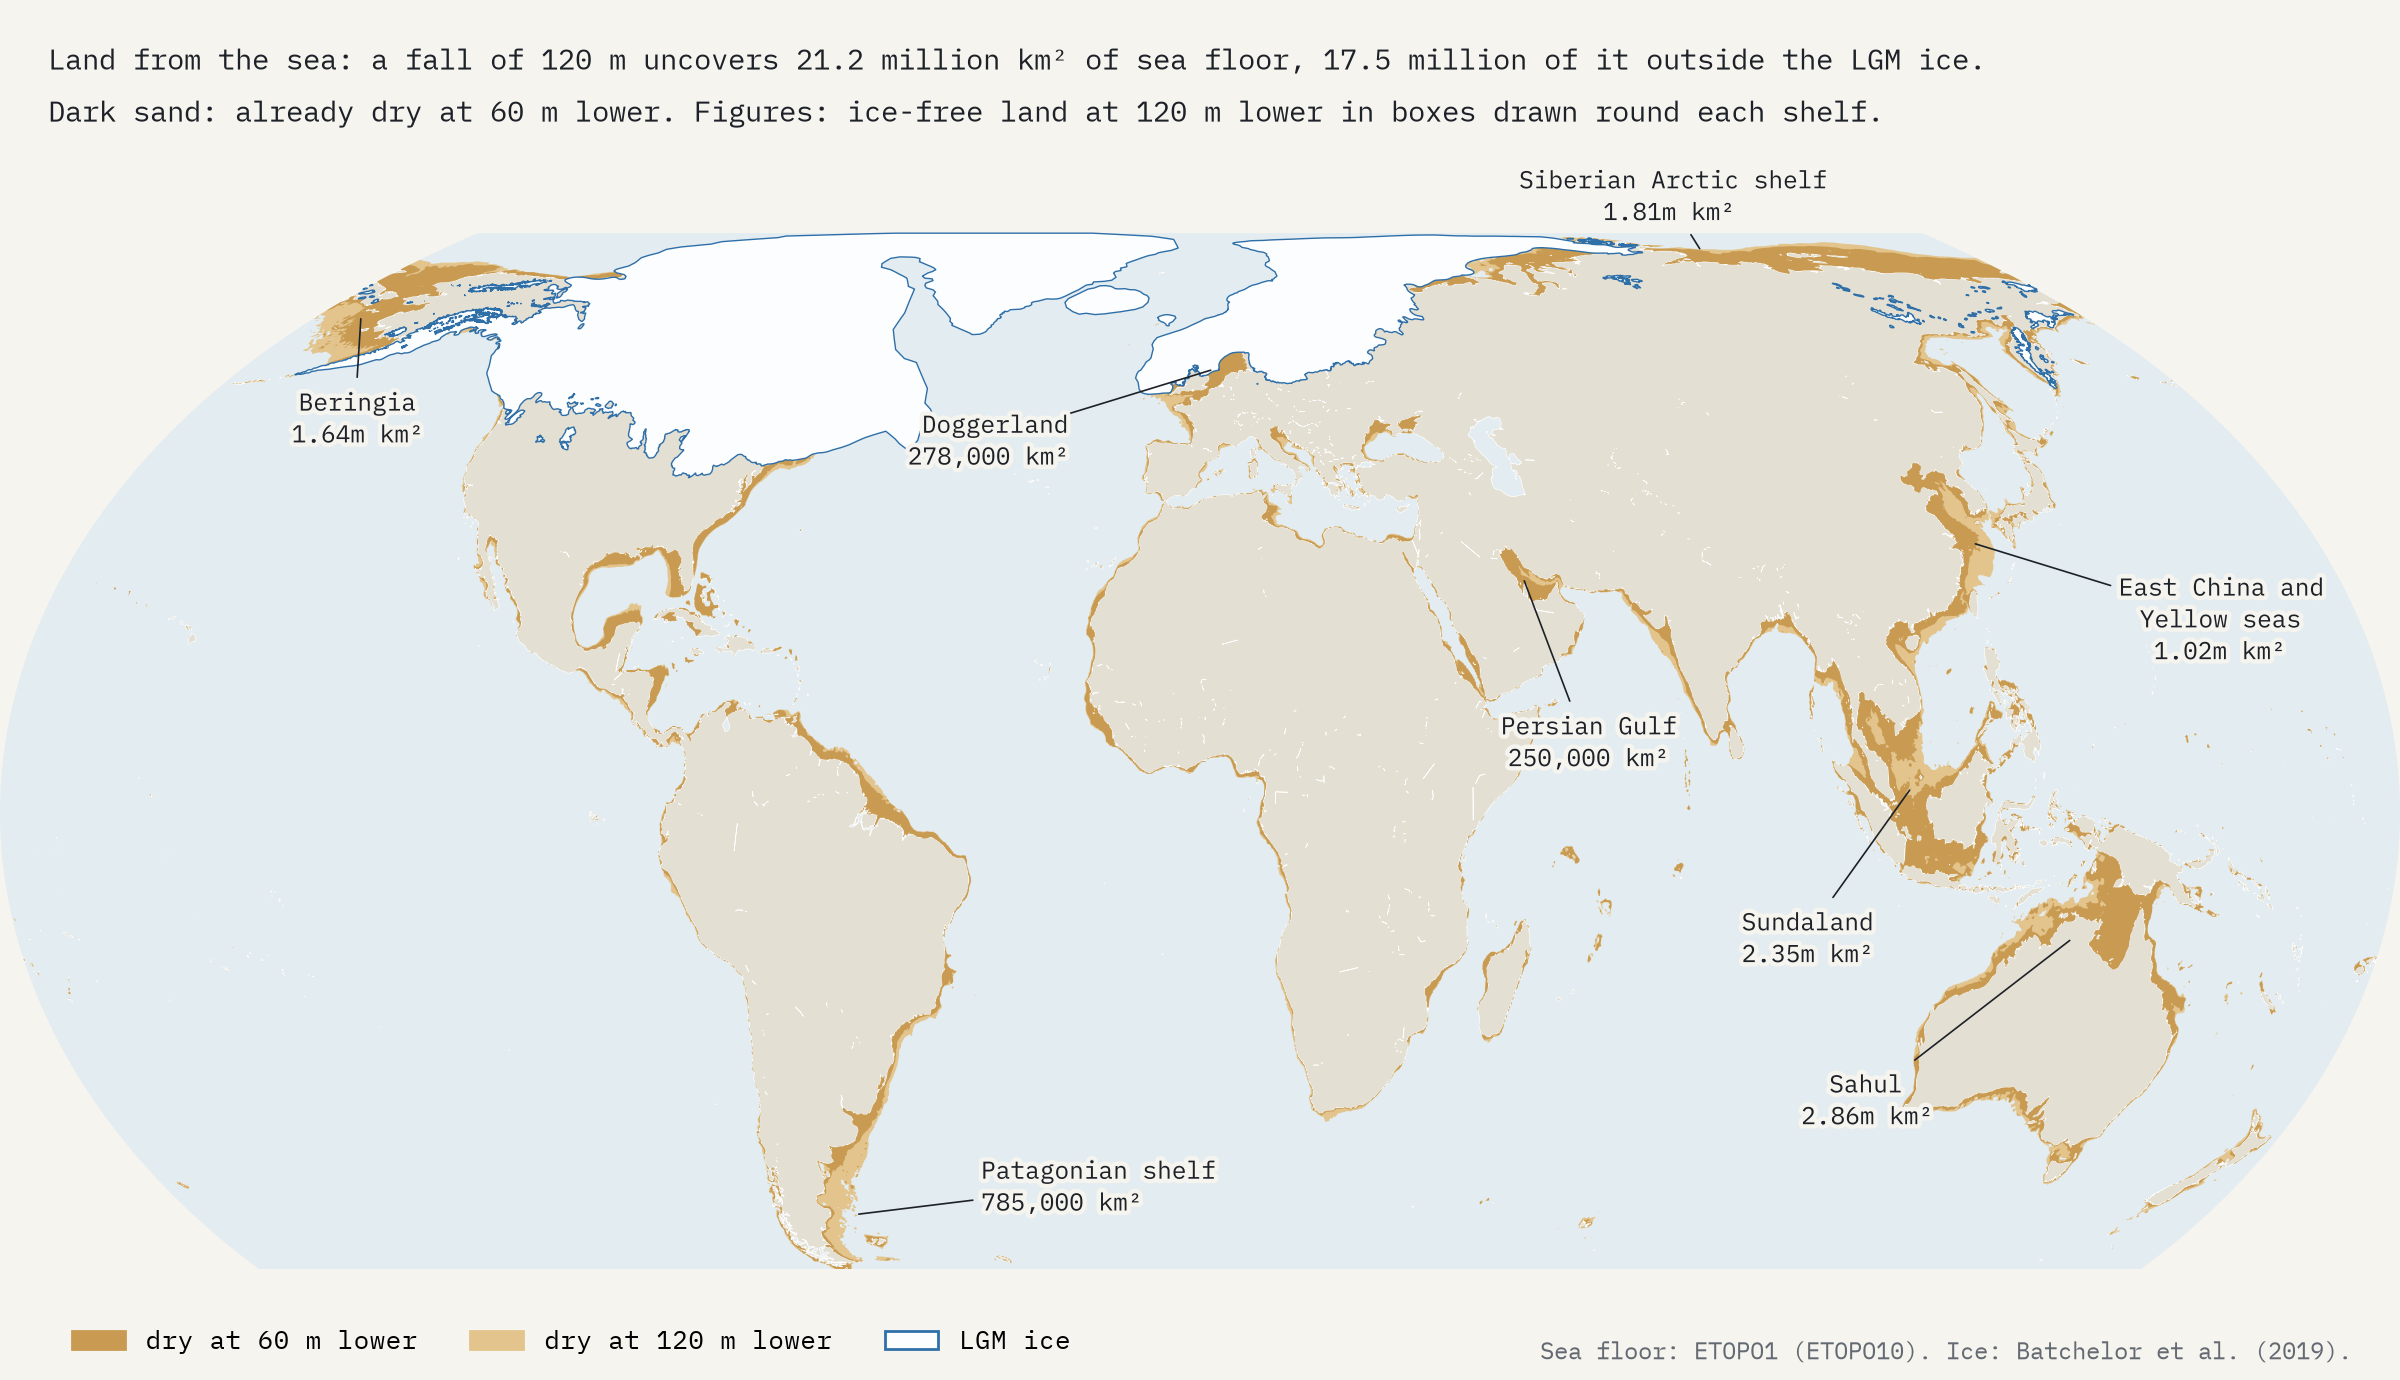
\includegraphics[width=\textwidth]{f_exposed.png}
\caption{Sea floor exposed by sea levels 60 m and 120 m below today's, with the LGM ice, and ice-free exposed area in the shelf boxes.}\label{fig:exposed}\end{figure}

\section{Limitations}
First, the outlines are generalised, partly subjective reconstructions of the maximum extent within each slice, compiled from evidence of very uneven density; they are not meant for local use, and the older slices are much less certain than the LGM, as the width of the authors' minimum to maximum ranges shows. Second, each slice's ice need not have reached its limits everywhere at once. Third, two files carry unrelated present-day glaciers that I removed only south of the equator, so small Northern Hemisphere glaciers remain in those two slices. Fourth, populations are Natural Earth's figures for named places and are indicative only. Fifth, the exposed-land figures use a fixed sea level on today's sea floor, at a resolution of about 18 km, without isostasy, sediment or the timing of each slice's lowstand, and the shelf boxes are my own.

\section{Conclusion}
In the reconstructions of \citet{batchelor}, the Last Glacial Maximum is a large but not exceptional Quaternary glaciation: MIS 6, MIS 12 and MIS 16 each had more ice, and the older ice reached further south, to southern Illinois and the Dnieper and Don valleys. The ice of the LGM alone lay over land where hundreds of cities stand today, from New York and Chicago to Berlin and St Petersburg, while London, Paris and Prague stayed clear of every outline. The water locked in that ice uncovered some 17.5 million \kmq\ of ice-free land, most of it in the tropics and the Arctic, and joined Britain to Europe, Asia to America and Australia to New Guinea.

\section*{Data and code availability}
The interactive map is at \url{https://maps.tristanhotham.com/ice-ages/}. Data and code are at \url{https://github.com/Tristan-Hotham/ice-ages} and archived with this paper at https://doi.org/10.5281/zenodo.23878610. Derived data and text are released under CC BY 4.0 and code under the MIT licence. The ice outlines are those of \citet{batchelor} (CC BY 4.0); please cite their paper.

\section*{AI statement}
I wrote the text, with drafting and editing assistance from Claude (Anthropic), which also helped prepare the analysis code. I reviewed and checked all text and results.

\begin{thebibliography}{9}
\bibitem[Batchelor et al.(2019)]{batchelor} Batchelor, C.L., Margold, M., Krapp, M., Murton, D.K., Dalton, A.S., Gibbard, P.L., Stokes, C.R., Murton, J.B. and Manica, A. (2019) The configuration of Northern Hemisphere ice sheets through the Quaternary. \textit{Nature Communications} 10, 3713. doi:10.1038/s41467-019-11601-2. Data: \url{https://osf.io/7jen3/}, CC BY 4.0.
\bibitem[Ehlers et al.(2011)]{ehlers} Ehlers, J., Gibbard, P.L. and Hughes, P.D. (eds) (2011) \textit{Quaternary Glaciations: Extent and Chronology, a Closer Look}. Developments in Quaternary Science 15. Elsevier. (As cited by Batchelor et al. 2019 for the LGM outline.)
\bibitem[Amante and Eakins(2009)]{etopo1} Amante, C. and Eakins, B.W. (2009) ETOPO1 1 Arc-Minute Global Relief Model: Procedures, Data Sources and Analysis. NOAA Technical Memorandum NESDIS NGDC-24. doi:10.7289/V5C8276M. Used through ETOPO10 by G. Euler (MIT licence).
\bibitem[Natural Earth(2026)]{naturalearth} Natural Earth (2026) Admin 0 countries, land and populated places, 1:10m and 1:50m. Public domain. \url{https://www.naturalearthdata.com/}
\bibitem[Wikipedia(2026)]{wiki} Wikipedia contributors (2026) Last Glacial Maximum (revision 1383210217), Quaternary glaciation (revision 1382049061), Beringia (revision 1375387022), Sundaland (revision 1382038749), Sahul (revision 1382059199), Doggerland (revision 1383229163). English Wikipedia, CC BY-SA 4.0.
\end{thebibliography}
\end{document}
